\documentclass[12pt]{article}
\usepackage{multicol,graphicx}
\usepackage[colorlinks,breaklinks,linkcolor=red,citecolor=blue]
{hyperref} 
\def\sectionautorefname~#1\null{\S#1\null}
\usepackage{charter,amsmath,amssymb,breakurl}
\usepackage{eulervm}
\usepackage[letterpaper,margin=.75in]{geometry}
\def\equationautorefname~#1\null{(#1)\null}
\def\itemautorefname~#1\null{(#1)\null}
\title{Worksheet 4}
\author{}\date{}
\let\ln\relax\DeclareMathOperator{\ln}{\mathsf{ln}}
\let\sin\relax\DeclareMathOperator{\sin}{\mathsf{sin}}
\let\arctan\relax\DeclareMathOperator{\arctan}{\mathsf{arctan}}
\let\cos\relax\DeclareMathOperator{\cos}{\mathsf{cos}}
\let\sec\relax\DeclareMathOperator{\sec}{\mathsf{sec}}
\let\min\relax\DeclareMathOperator*{\min}{\mathsf{min}}
\let\max\relax\DeclareMathOperator*{\max}{\mathsf{max}}
\let\sup\relax\DeclareMathOperator*{\sup}{\mathsf{sup}}
\let\inf\relax\DeclareMathOperator*{\inf}{\mathsf{inf}}
\let\lim\relax\DeclareMathOperator*{\lim}{\mathsf{lim}}
\everymath{\displaystyle}
\begin{document}
\maketitle
\thispagestyle{empty}

\begin{enumerate}
\item Set up an integral to calculate
the area of the crescent moon formed by
the circles $x^2+y^2=9$ and $\left(x+4\right)^2+y^2=25$
by following the following steps.
\begin{enumerate}
\item Write polar equations for both circles.
\item Solve both equations for $r$ in terms of $\theta$. This
will involve the quadratic formula.
\item Set up (but don't necessarily evaluate)
a double integral to find the area
of the moon.
\end{enumerate}

\item Evaluate the integral
$\int_0^1\int_0^{\sqrt{1-x^2}}\int_0^{\sqrt{x^2+y^2}}
\left(z+\sqrt{x^2+y^2}\right)dzdydx$.

\item Find the mass of the triangular plate with vertices
$\left(0,4\right)$, $\left(4,0\right)$, $\left(-2,0\right)$
whose density at $\left(x,y\right)$ is $\delta\left(x,y\right)
=y~\mathsf{g}/\mathsf{m}^2$.

\item Let $W$ be the solid sphere bounded by $x^2+y^2+z^2=1$.
Decide without calculation whether each integral below
is positive, negative or zero.
\begin{enumerate}
\item $\int_WzdV$
\item $\int_WxydV$
\item $\int_W\sin\left(\frac{\pi xy}{2}\right)dV$
\item $\int_W\left(z^2-1\right)dV$
\item $\int_W\sqrt{x^2+y^2+z^2}dV$
\end{enumerate}

\item Set up an iterated integral to evaluate
$\int_Rf\left(x,y,z\right)dV$ where $R$ is
the region below the plane $z=x+2y$ and inside
the unit cube $-1\le x,y,z\le 1$. Use the volume
element $dzdydx$.

\item A bead is made by drilling a cylindrical
hole of radius $1~\mathsf{mm}$ through a sphere
of radius $5~\mathsf{mm}$. Set up and evaluate
a triple integral to find the volume of the bead.

\item A half-melon is approximated by the region
between two concentric spheres, one of radius~$a$
and the other of radius~$b$, with $0<a<b$. Write
and evaluate a triple integral giving the volume
of the half-melon.

\item Evaluate the integral
$\int_0^1\int_y^1\sin\left(x^2\right)dxdy$.

\end{enumerate}

{\bf Answers:}
\begin{enumerate}
\item\begin{enumerate}
\item $r^2+8r\cos{\theta}=9$ and $r=3$
\item $r=-4\cos{\theta}+\sqrt{16\cos^2{\theta}+9}$ and $r=3$
\item The two curves intersect where $\theta=\pm\frac{\pi}{2}$ so the
area is given by \[\int_{-\pi/2}^{\pi/2}\int
_{-4\cos{\theta}+\sqrt{16\cos^2{\theta}+9}}^3r\;drd\theta\approx 10\]
\end{enumerate}
\item $\int_0^{\pi/2}\int_0^1\int_0^r
\left(zr+r^2\right)\; drdzd\theta=\frac{3\pi}{16}$
\item $\int_0^4\int_{\frac{y}{2}-2}^{4-y}y\;dxdy=16$
\item Zero, zero, zero, negative, positive
\item
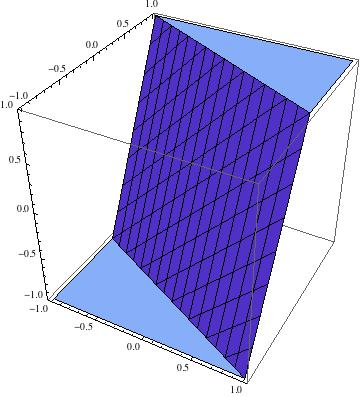
\includegraphics[scale=.5]{PlaneDensity}
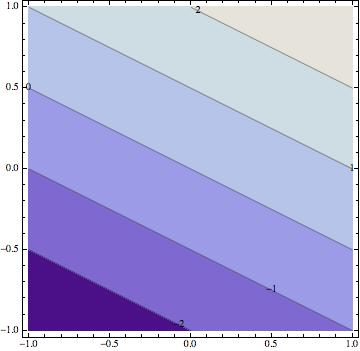
\includegraphics[scale=.5]{ContourPlane}\\
 $\int_{-1}^1\int_{-\frac{1}{2}-\frac{x}{2}}
^{\frac{1}{2}-\frac{x}{2}}\int_{-1}^{x+2y}
f\left(x,y,z\right)dzdydx
+\int_{-1}^1\int_{\frac{1}{2}-\frac{x}{2}}
^1\int_{-1}^1
f\left(x,y,z\right)dzdydx$
\item $\int_0^{2\pi}\int_1^5\int_{-\sqrt{25-r^2}}
^{\sqrt{25-r^2}}r\;dzdrd\theta=64\sqrt{6}\pi$
\item $\int_0^{2\pi}\int_0^{\pi/2}\int_a^b\rho^2\sin{\phi}
d\rho d\phi d\theta=2\pi\frac{b^3-a^3}{3}$
\item $\frac{1-\cos{1}}{2}$
\end{enumerate}
\end{document}
